
\section{Results}\label{sec:results}                           %% The first section





\subsection{River2D Modelling}\label{sec:river2d}       




The software program River2D was used to calculate the habitat suitability in a section of the River Ybbs. First a model was created of the River Ybbs. A file containing habitat suitability parameters of brown trout at different age classes was prepared. Choriope information was also entered into River2D. The software then calculated the weighted usable area (WUA) for the age classes at different flow rates (\SI[per-mode=symbol]{0.35}{\cubic\meter\per\second} - \SI[per-mode=symbol]{2.16}{\cubic\meter\per\second} - \SI[per-mode=symbol]{6.00}{\cubic\meter\per\second} - \SI[per-mode=symbol]{13.00}{\cubic\meter\per\second} - \SI[per-mode=symbol]{20.00}{\cubic\meter\per\second}). \cref{fig:flow_rate_age_class} shows the total WUA of age classes at each flow rate. The 0+ fish have a much higher WUA at low flows, while the larger 2+ fish have almost no WUA at \SI[per-mode=symbol]{0.35}{\cubic\meter\per\second} flow.


\begin{figure}[!htb] 
	\centering
	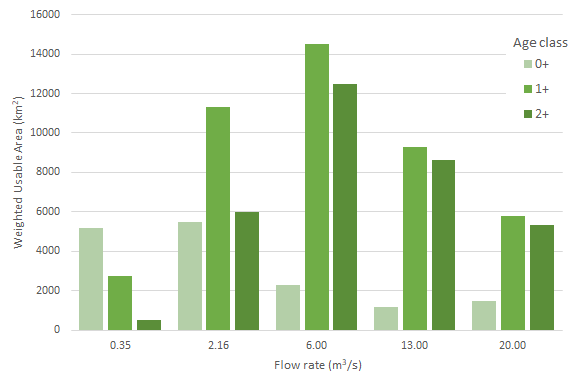
\includegraphics[width=.8\textwidth]{images/flow_rate_age_class}
	\caption{Total weighted usable area by age class and flow rate in the River Ybbs for brown trout as calculated by River2D.}\label{fig:flow_rate_age_class}
\end{figure}

River2D was then used to create maps of the Ybbs showing the combined suitabilty for each age class. At \SI[per-mode=symbol]{0.35}{\cubic\meter\per\second}, adult brown trout have very limited habitat available, thus habitat suitability is very low (\cref{fig:2_0035}). Conversely, \cref{fig:2_0600} shows that a flow rate of \SI[per-mode=symbol]{6.00}{\cubic\meter\per\second} provides an abundance of habitat and near ideal conditions for adult brown trout. See the~\hyperref[appendixA]{Appendices} for the collection of maps representing the combined suitability of all brown trout age classes at different flow rates. 


\begin{figure}[!htb] 
	\centering
	\begin{subfigure}{.3\textwidth}
		\centering
		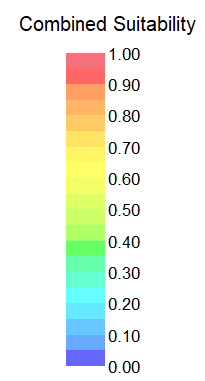
\includegraphics[width=.9\linewidth]{images/suitability_index}
	\end{subfigure}%
	\begin{subfigure}{.7\textwidth}
		\centering
		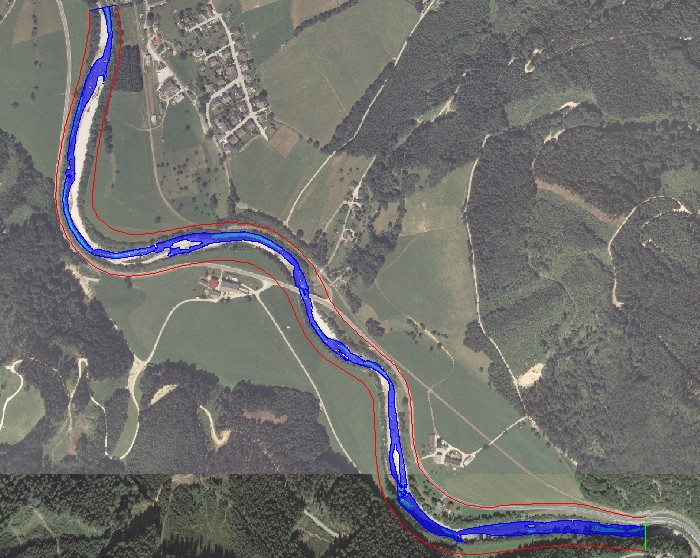
\includegraphics[width=\linewidth]{images/2_0035}
	\end{subfigure}
	\caption{Brown trout (2+ class) combined suitability at \SI[per-mode=symbol]{0.35}{\cubic\meter\per\second}.}
	\label{fig:2_0035}
\end{figure}


\begin{figure}[!htb] 
	\centering
	\begin{subfigure}{.3\textwidth}
		\centering
		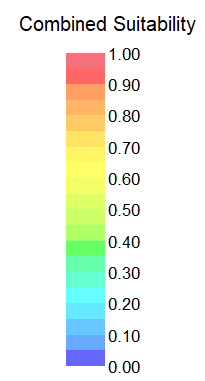
\includegraphics[width=.7\linewidth]{images/suitability_index}
	\end{subfigure}%
	\begin{subfigure}{.7\textwidth}
		\centering
		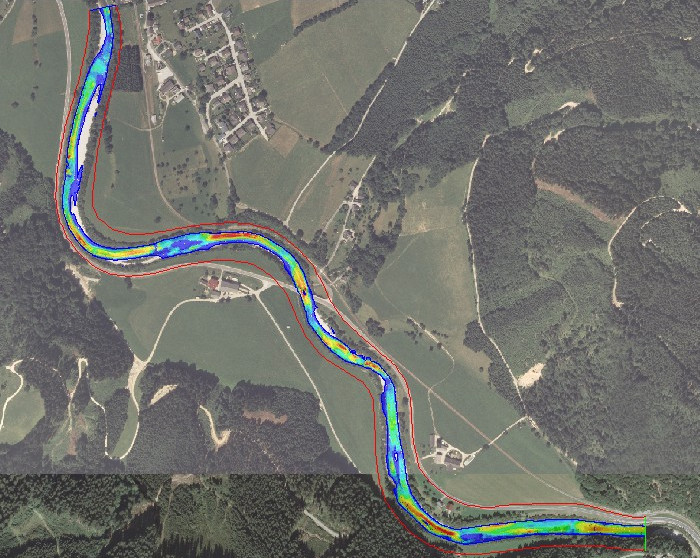
\includegraphics[width=\linewidth]{images/2_0600}
	\end{subfigure}
	\caption{Brown trout (2+ class) combined suitability at \SI[per-mode=symbol]{6.00}{\cubic\meter\per\second}.}
	\label{fig:2_0600}
\end{figure}



\begin{figure}[!htb]                                                        	%% SI depth
	
	\centering                                                                  	%% Center the figures
	\hfill
	\subcaptionbox{Depth SI for 1+\label{fig:SI_depth_1}}{   	%% First subcaption
		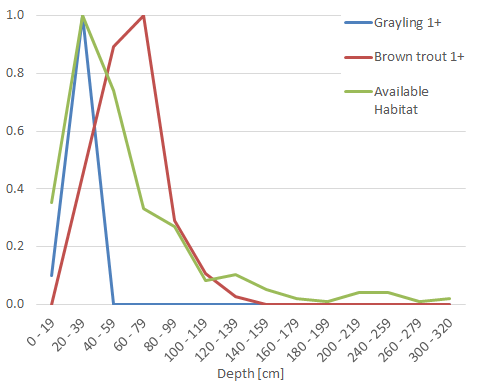
\includegraphics[width=0.48\columnwidth]{images/SI_depth_1}}   						%% Set width and select first image COLOR
	\hfill                                                                   		%% Fill Blank space
	\subcaptionbox{Depth SI for 2+\label{fig:SI_depth_2}}{    %% Second subcaption
		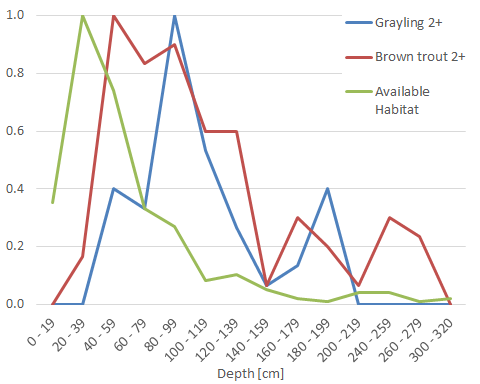
\includegraphics[width=0.48\columnwidth]{images/SI_depth_2}}        				%% Set width and second image COLOR
	\hspace*{\fill}                                                                         %% Fill blank space
	\hfill
	\subcaptionbox{Mean velocity SI for 1+\label{fig:SI_vmean_1}}{   	%% First subcaption
		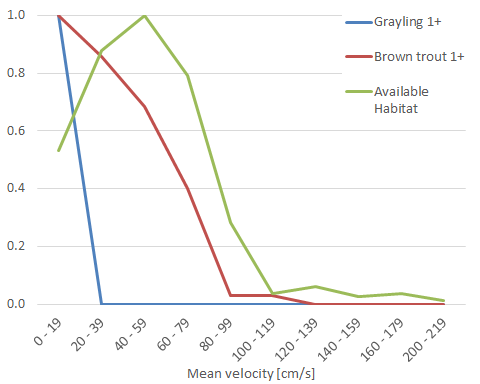
\includegraphics[width=0.48\columnwidth]{images/SI_vmean_1}}   						%% Set width and select first image COLOR
	\hfill                                                                   		%% Fill Blank space
	\subcaptionbox{Mean velocity for 2+\label{fig:SI_vmean_2}}{    %% Second subcaption
		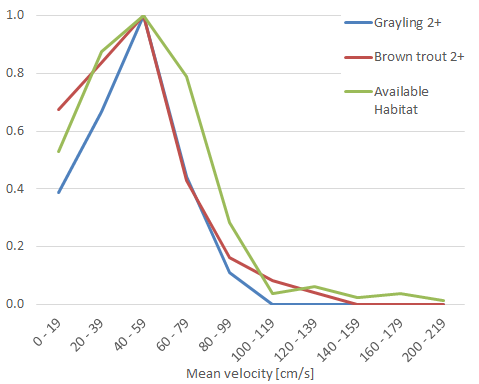
\includegraphics[width=0.48\columnwidth]{images/SI_vmean_2}}        				%% Set width and second image COLOR
	\hspace*{\fill}                                                                         %% Fill blank space
	
	\caption{Calculated habitat suitability index ratings (SI) of different age classes by depth and mean velocity from the sampled area of the Ois River.}\label{fig:SI_depth}        %% Capition for both figures
\end{figure}


























